\documentclass[12pt]{article} % use larger type; default would be 10pt
\usepackage[utf8]{inputenc} % set input encoding (not needed with XeLaTeX)

%%% PAGE DIMENSIONS
\usepackage{geometry} % to change the page dimensions
\geometry{a4paper} % or letterpaper (US) or a5paper or....
\geometry{margin=2cm} % or letterpaper (US) or a5paper or....

\usepackage{graphicx} % support the \includegraphics command and options
\usepackage[parfill]{parskip} % Activate to begin paragraphs with an empty line rather than an indent
\usepackage{times} % for Times Roman default font

%%% PACKAGES
\usepackage{booktabs} % for much better looking tables
\usepackage{array} % for better arrays (eg matrices) in maths
\usepackage{paralist} % very flexible & customisable lists (eg. enumerate/itemize, etc.)
\usepackage{verbatim} % adds environment for commenting out blocks of text & for better verbatim
\usepackage{subfig} % make it possible to include more than one captioned figure/table in a single float

%%% HEADERS & FOOTERS
\usepackage{fancyhdr} % This should be set AFTER setting up the page geometry
\pagestyle{fancy} % options: empty , plain , fancy
\renewcommand{\headrulewidth}{0pt} % customise the layout...
\lhead{}\chead{}\rhead{}
\lfoot{}\cfoot{\thepage}\rfoot{}

\makeatletter
\renewcommand{\maketitle}{%
  {\bfseries{\scshape{\Large{\@title\par}}}}
}
\makeatother

\hyphenation{Kiwi-bank} % otherwise it may get hyphenated as Ki-wibank

%%% END Article customizations

%%% The "real" document content comes below...

\title{Boyle Flats Hut: 14-15 August 2017}

\begin{document}
  \maketitle
Leaving from Boyle Village we crossed the over the swing bridge after a bit more than half an hour, and continued for another hour or so before stopping for lunch (we didn't start walking until shortly after 11:00).  It was then another hour or so to the next bridge and the turn-off to Magdalen Hut.  From here another hour saw us at the hut (i.e., a bit over 3$\frac{1}{2}$ hours total, \textit{cf} 4$\frac{1}{2}$ track time).

Boyle Flats Hut is fairly large, but the fire puts out good heat and we were able to get it warmish (14$^o$C whereas it was about 7$^o$C on arrival).  There is a permolat-marked track heading up behind the hut.  I only followed it a little way but it appeared to be well-defined and may lead up to the Libretto Range.  This would make a nice return route in more salubrious weather.

\begin{figure}[ht]
%\centering
\begin{minipage}{.5\linewidth}
\begin{flushleft}
   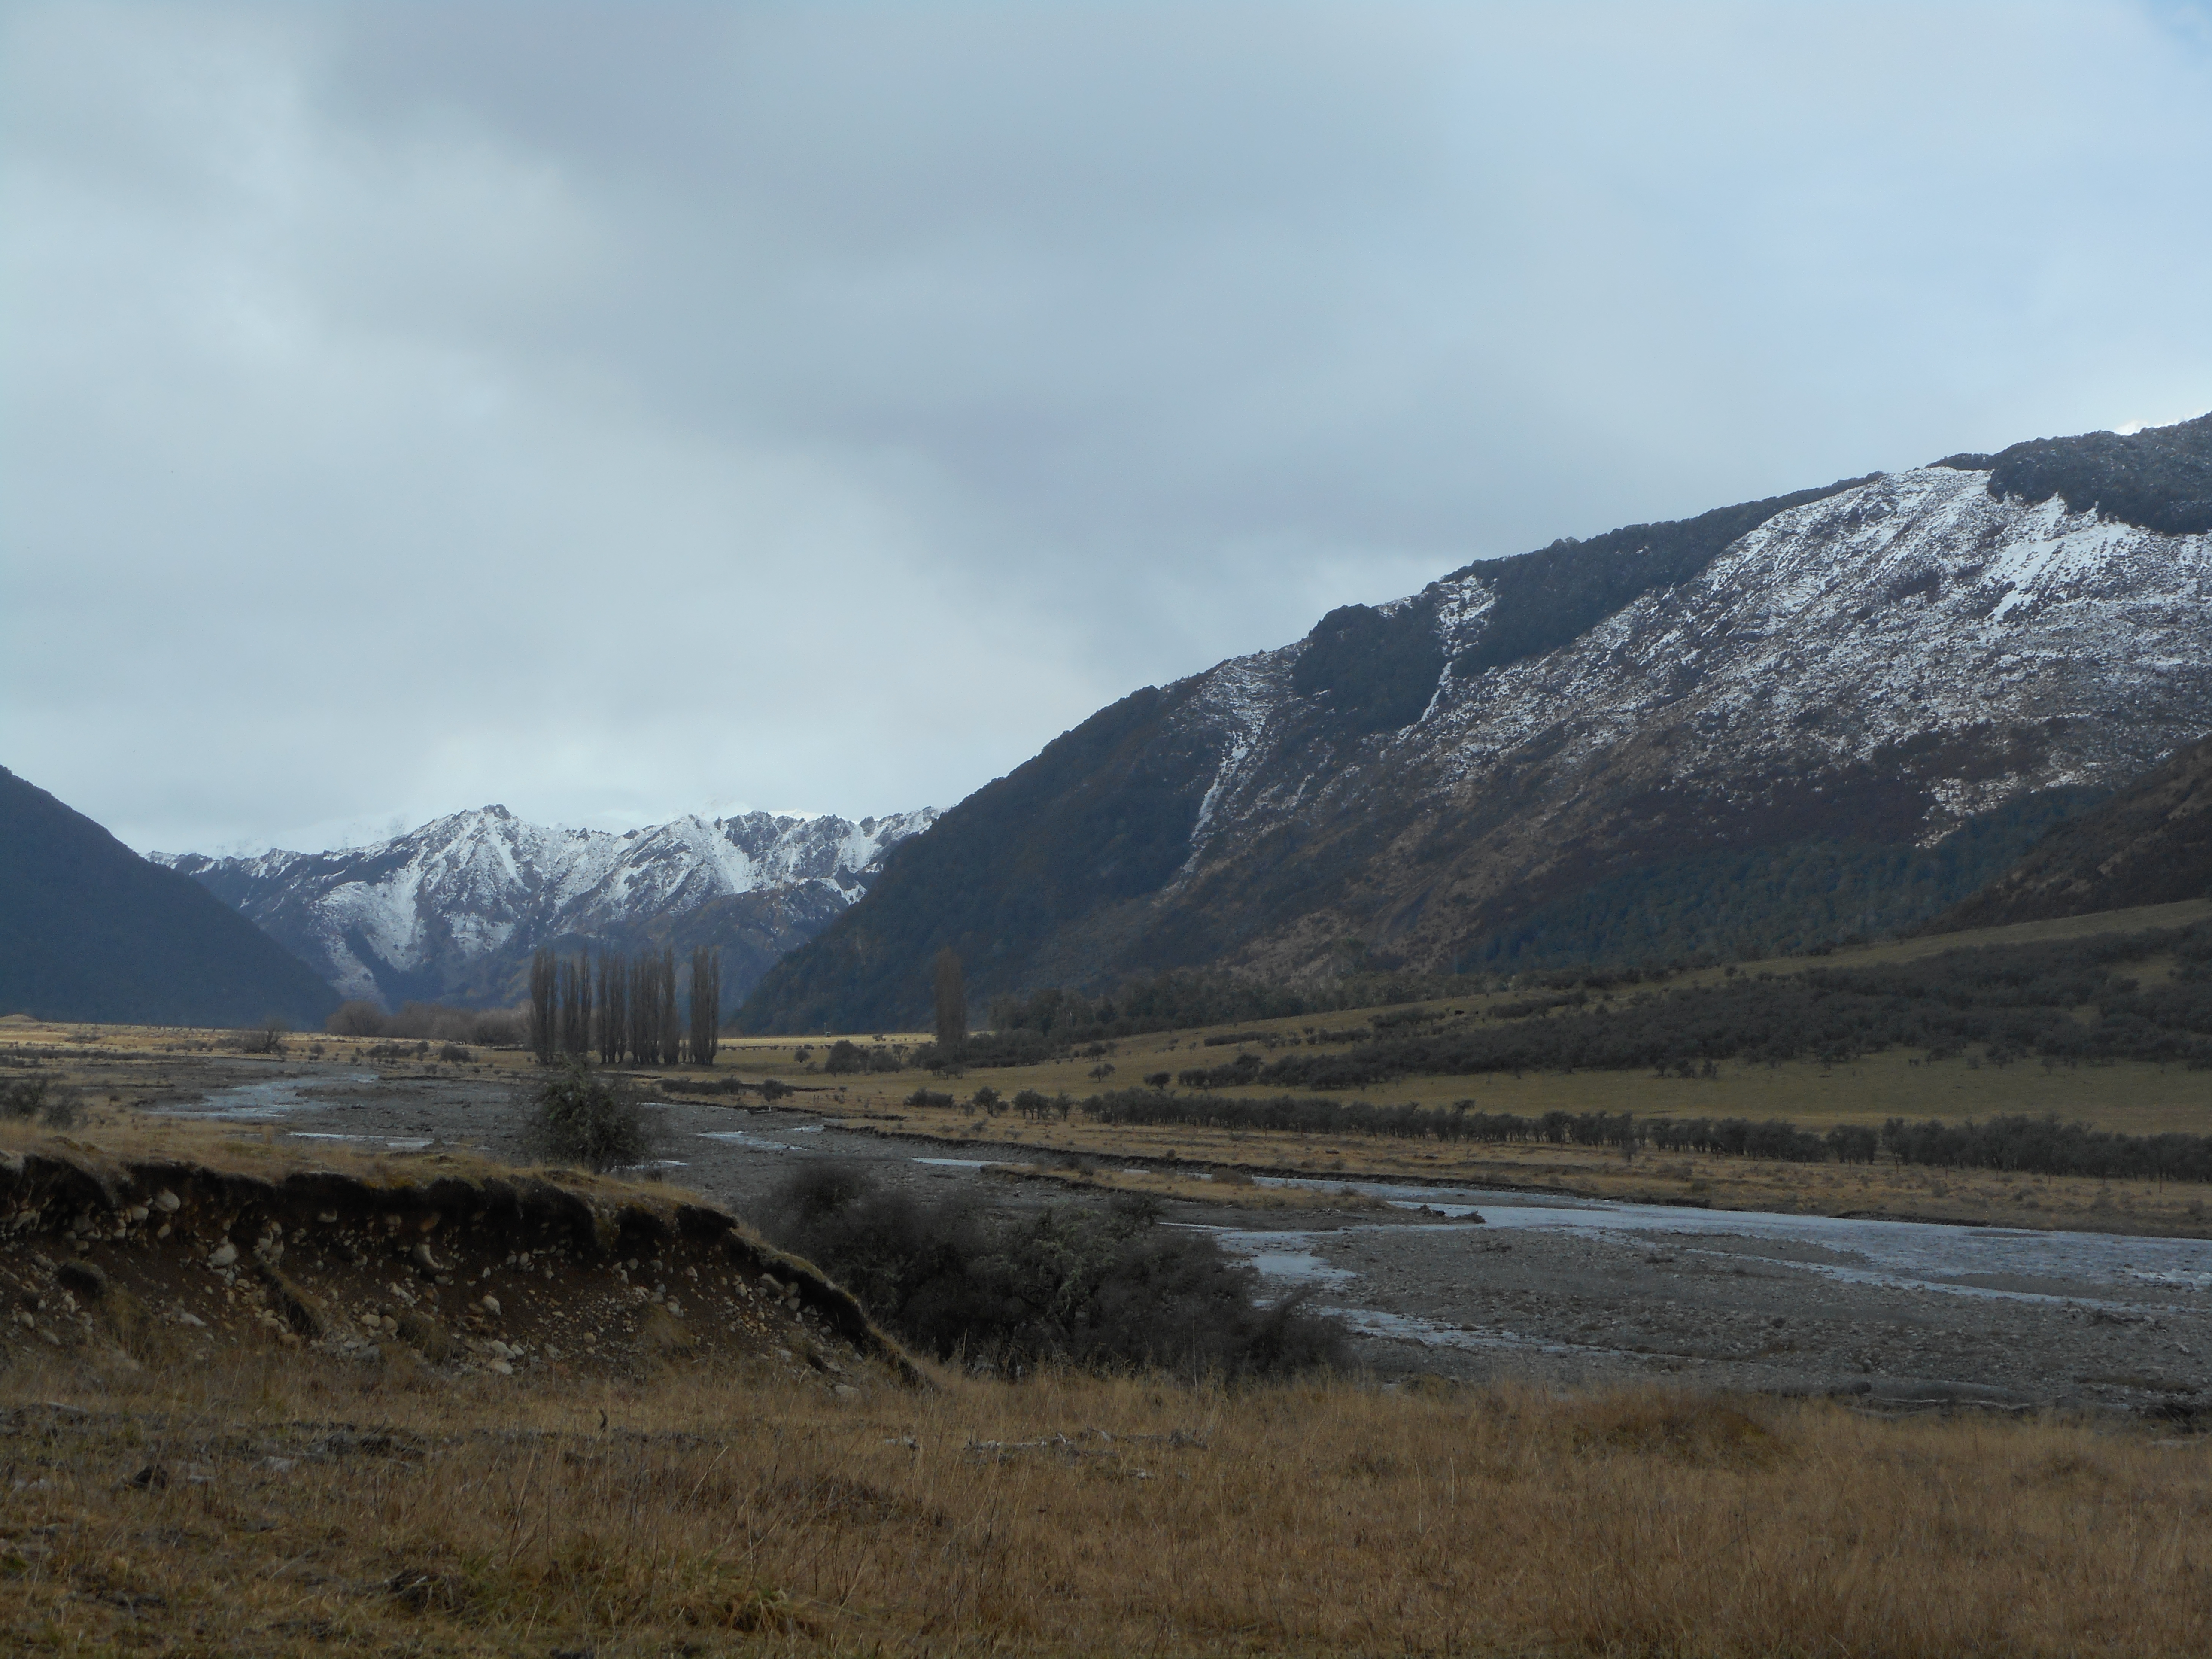
\includegraphics[width=8cm]{BoyleFlatsHut14Aug2017Photo1}
   \captionof{figure}{Boyle River}
\end{flushleft}
\end{minipage}
\begin{minipage}{.5\linewidth}
\begin{flushright}
   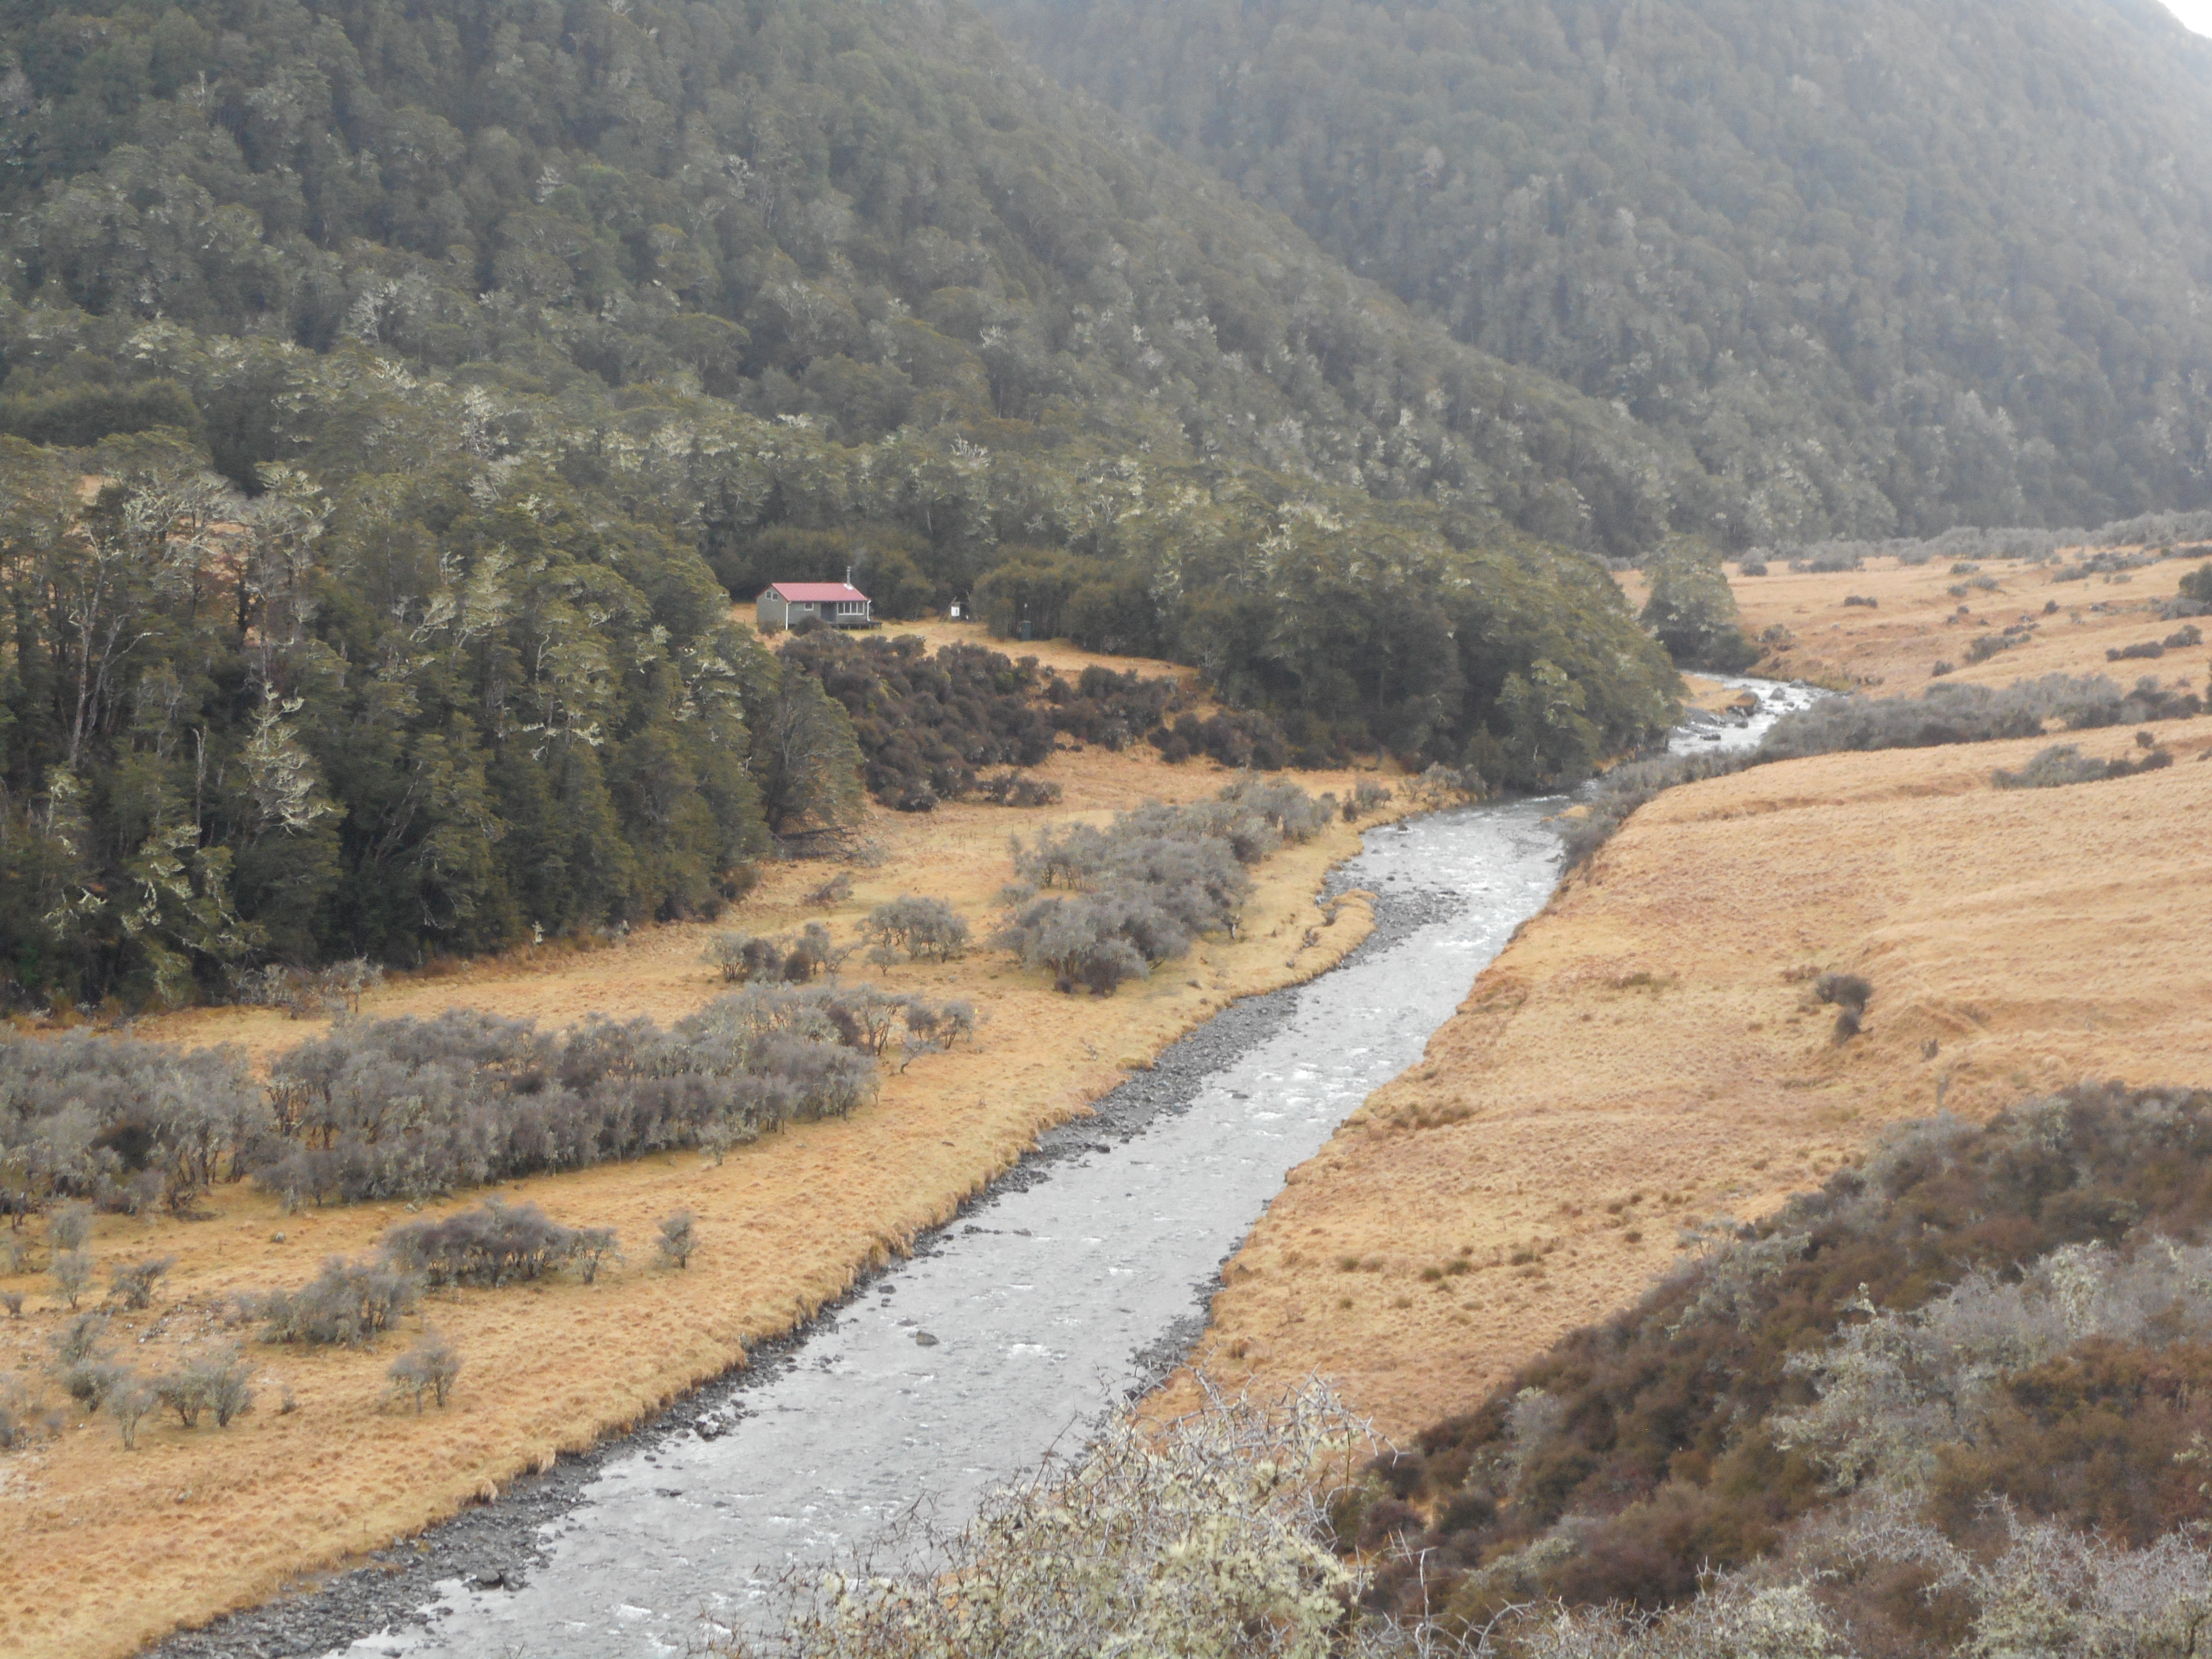
\includegraphics[width=8cm]{BoyleFlatsHut14Aug2017Photo2}
   \captionof{figure}{Boyle Flats Hut}
\end{flushright}
\end{minipage}
\end{figure}

On the way back we did a slight detour to Magdalen Hut (about 20 minutes each way, plus a further 20 minutes to explore).  This is a lovely new hut with double glazing, a free-standing fire and was well supplied with firewood.  Definitely worth another visit, as it would be very snug in winter.  Visitor numbers between May and November looked moderate.

\begin{figure}[ht]
%\centering
\begin{minipage}{.5\linewidth}
\begin{flushleft}
   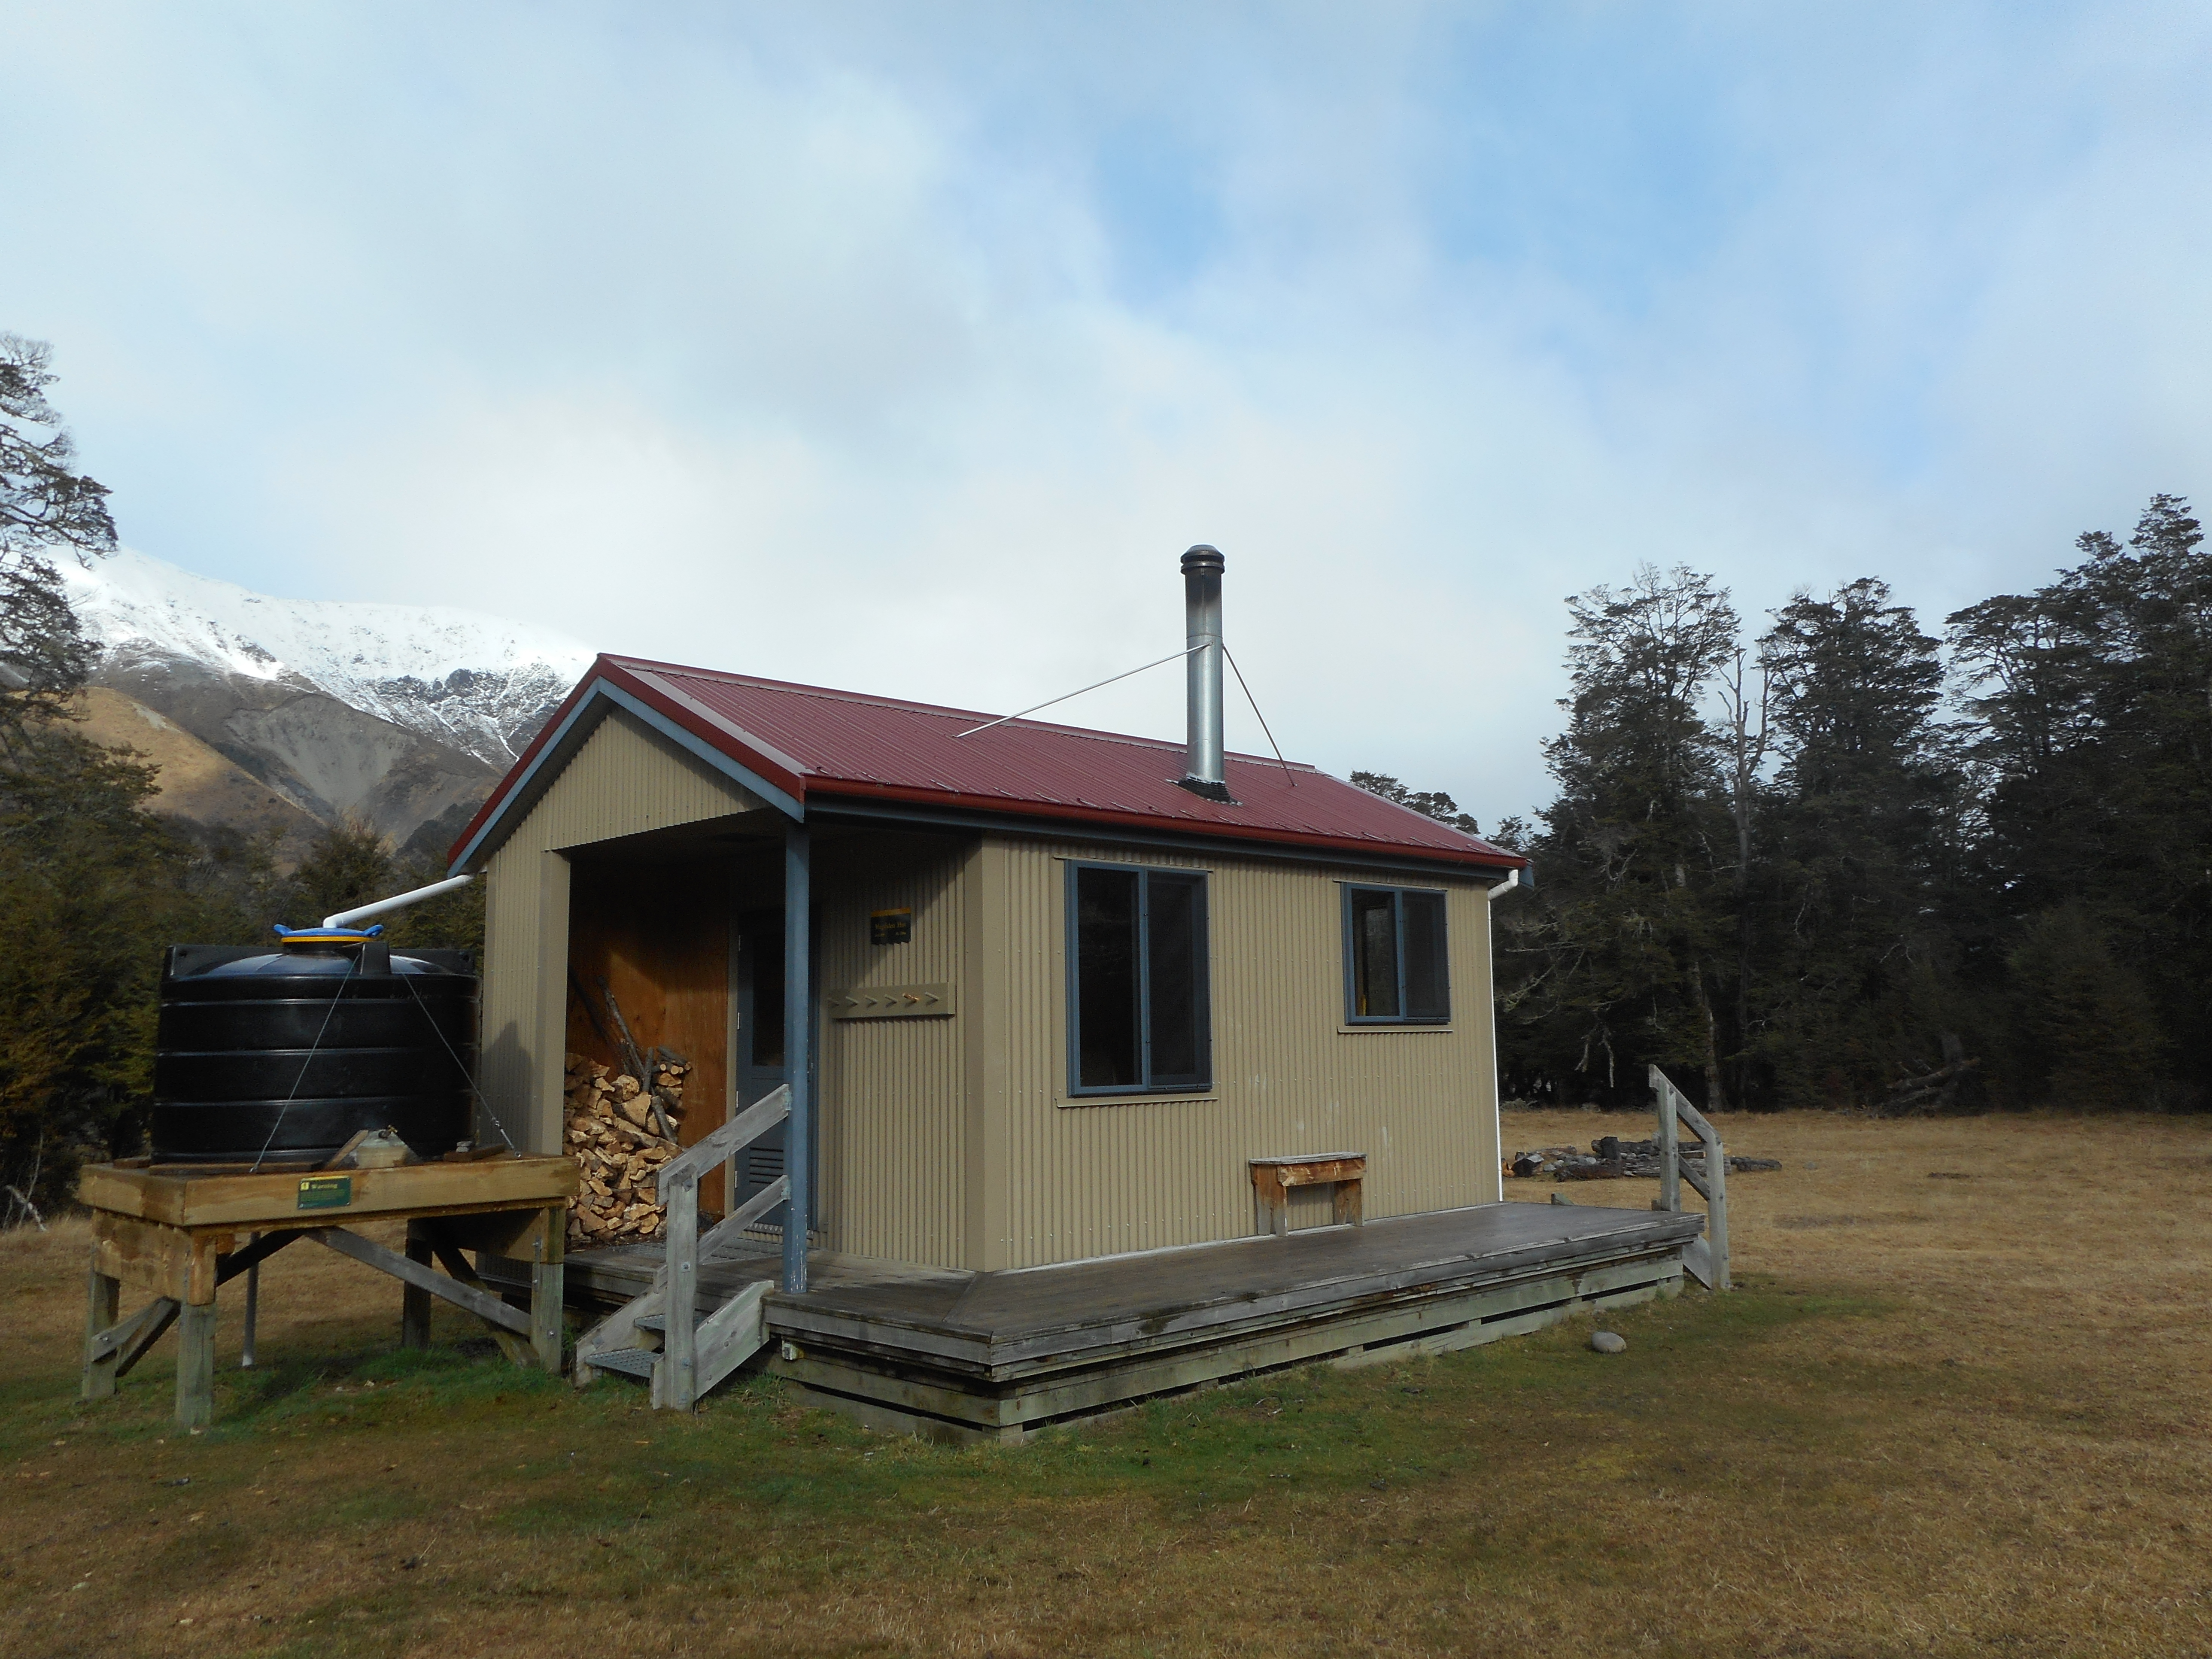
\includegraphics[width=8cm]{BoyleFlatsHut14Aug2017Photo3}
   \captionof{figure}{Magdalen Hut}
\end{flushleft}
\end{minipage}
\begin{minipage}{.5\linewidth}
\begin{flushright}
   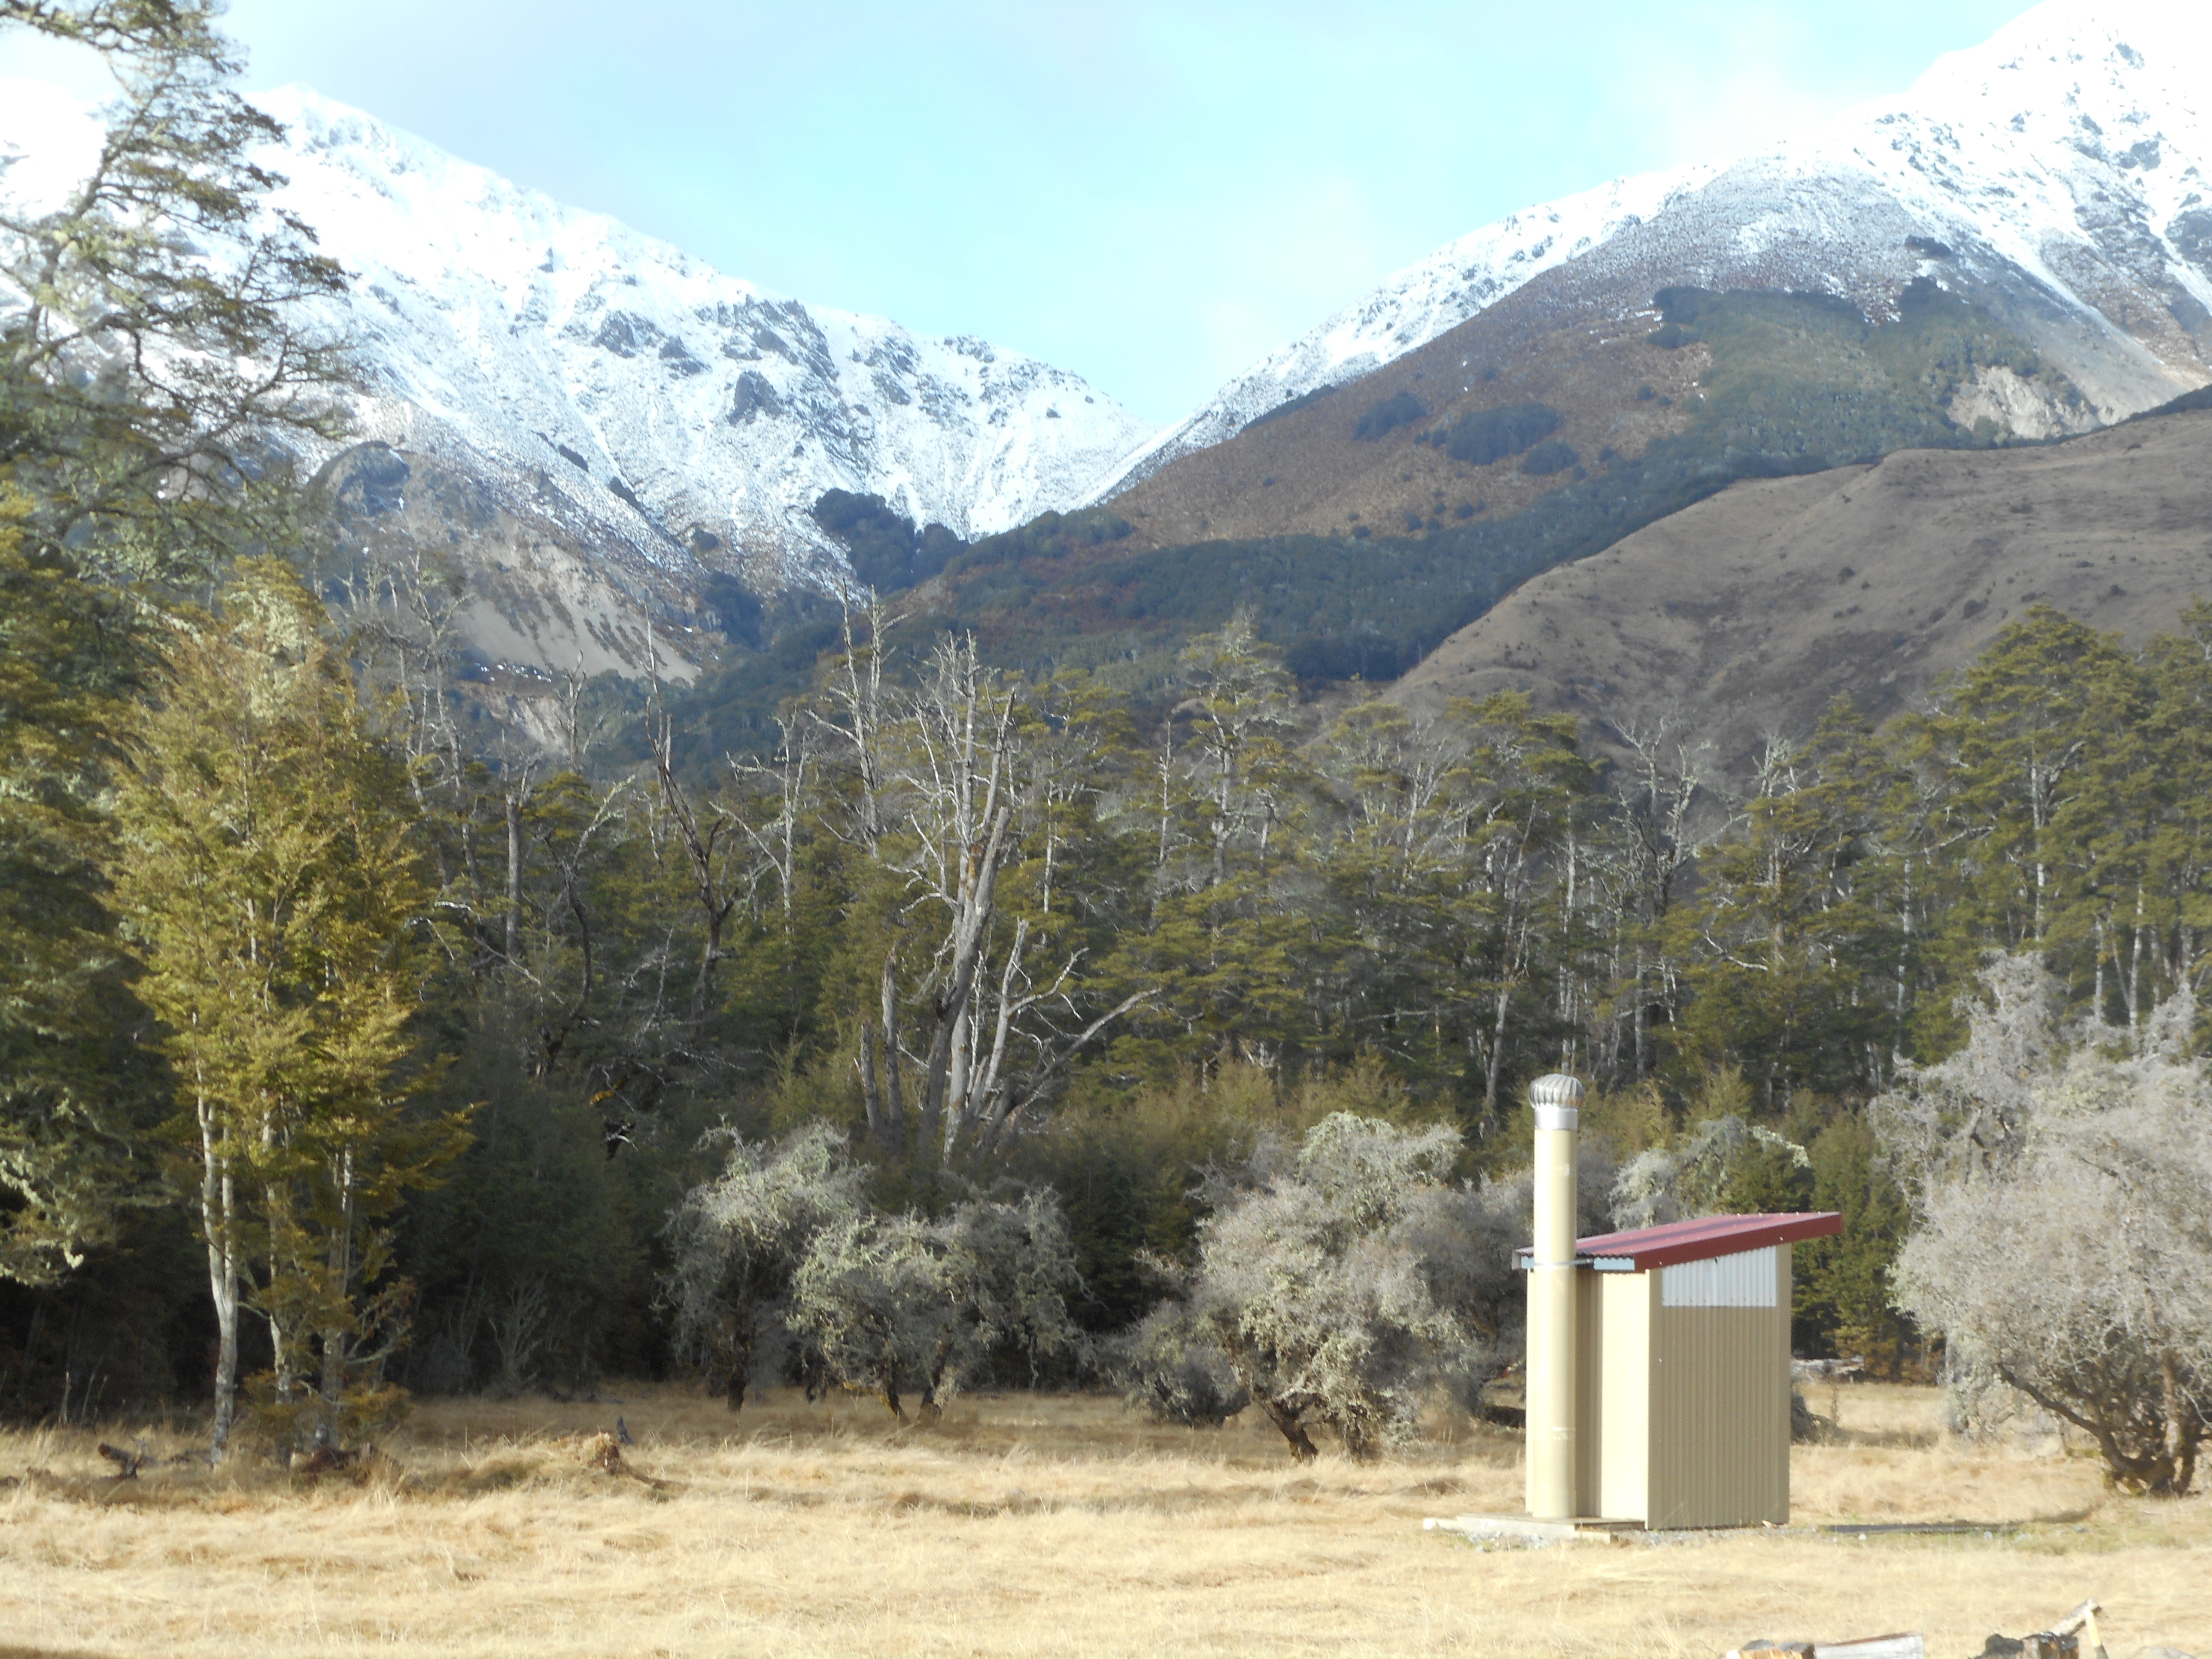
\includegraphics[width=8cm]{BoyleFlatsHut14Aug2017Photo4}
   \captionof{figure}{View from Magdalen Hut}
\end{flushright}
\end{minipage}
\end{figure}

\begin{flushright}
Robyn, Peter and dog
\end{flushright}

\end{document}
